% https://topanswers.xyz/tex?q=800#a941
\documentclass{beamer}
\usepackage{tikz}
\setbeamercovered{dynamic}

\begin{document}

\begin{frame}

\begin{figure}
	\includegraphics[width=2cm,page=1]{example-image-duck}
	Test A
	\pause
	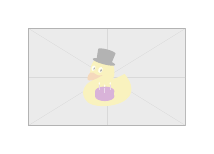
\begin{tikzpicture}
	\node[anchor=south west,inner sep=0] (B) at (4,0) {\includegraphics[width=2cm,page=2]{example-image-duck}};
	\only<1>{%
	    \fill [draw=none, fill=white, fill opacity=0.7] (B.north west) -- (B.north east) -- (B.south east) -- (B.south west) -- (B.north west) -- cycle;
	}
	\end{tikzpicture}
	Test B
	\pause	
	 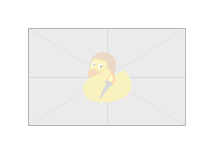
\begin{tikzpicture}
	    \node[anchor=south west,inner sep=0] (B) at (4,0) {\includegraphics[width=2cm,page=3]{example-image-duck}};
	    \only<1-2>{%
	        \fill [draw=none, fill=white, fill opacity=0.7] (B.north west) -- (B.north east) -- (B.south east) -- (B.south west) -- (B.north west) -- cycle;
	    }
	 \end{tikzpicture}	
	Test C
\end{figure}
\end{frame}

\end{document}